\documentclass{standalone}
\usepackage{tikz}
\usepackage{pgfplots}
\pgfplotsset{width=7cm,compat=1.8}
\usepgfplotslibrary{polar}

\title{Butterfly curve}
\begin{document}
	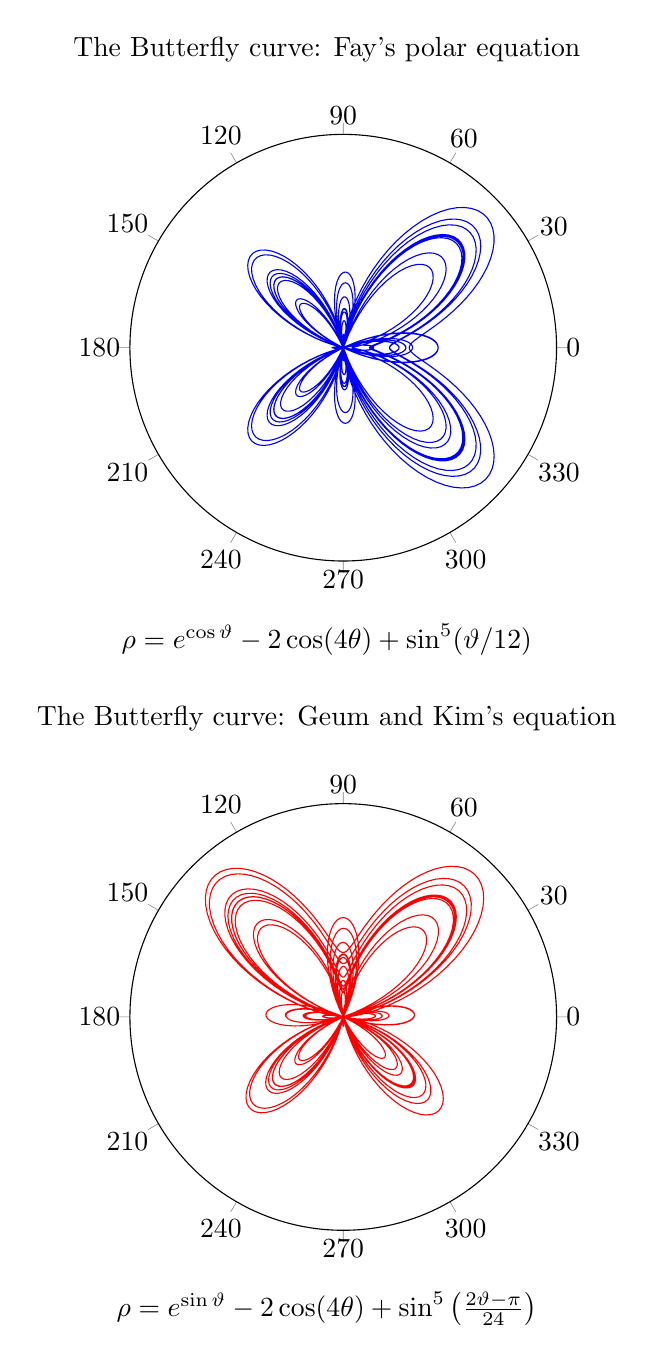
\begin{tikzpicture}
		\def\a{1}
		\def\b{4}
		\def\c{12}
		\def\A{2}
		\def\B{5}
		\def\pig{3.14}
		%
		\begin{scope}
			\node at (2.5,0) {The Butterfly curve: Fay's polar equation};
		\end{scope}
		%
		\begin{scope}[shift={(0,-6.5)}]
			\begin{polaraxis}[grid=none,hide y axis]
				\addplot+[mark=none,domain=0:3600,samples=2000] {e^cos(\a * x)-\A * cos(\b * x) + (sin(x / \c))^\B};
			\end{polaraxis}
			\node at (2.5,-1) {$\rho = e^{\cos \vartheta} - 2 \cos (4 \theta) + \sin^5 (\vartheta / 12)$};
		\end{scope}
		%
		\begin{scope}[shift={(0,-15)}]
			\node at (2.5,6.5) {The Butterfly curve: Geum and Kim's equation};
			\begin{polaraxis}[grid=none,hide y axis]
				\addplot+[mark=none,domain=0:3600,samples=2000,color=red] {e^sin(\a * x)-\A * cos(\b * x) + (sin((2*x - \pig)/ (2*\c)))^\B};
			\end{polaraxis}
			\node at (2.5,-1) {$\rho = e^{\sin \vartheta} - 2 \cos (4 \theta) + \sin^5 \left ( \frac{2\vartheta -\pi}{24} \right )$};
		\end{scope}
	\end{tikzpicture}
\end{document}